\documentclass[border=6pt]{standalone}
\usepackage[T1]{fontenc}
\usepackage{times}          % IEEE-style serif font
\usepackage{tikz}
\usetikzlibrary{arrows.meta, positioning, fit, backgrounds, calc,
                decorations.pathreplacing}
\begin{document}
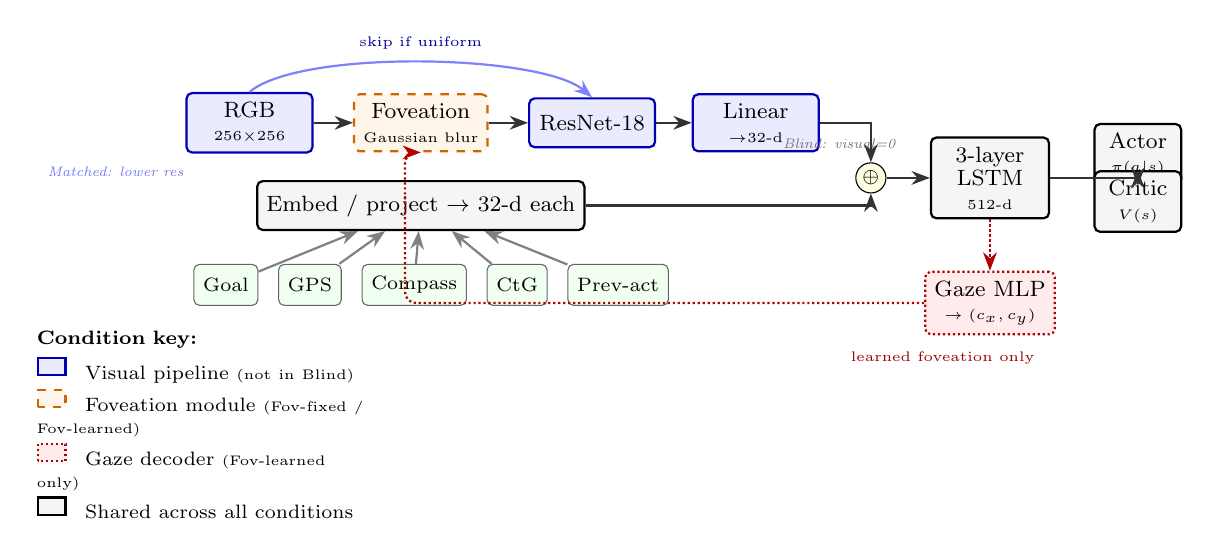
\begin{tikzpicture}[
    >=Stealth,
    node distance=0.45cm and 0.55cm,
    % --- block styles ---
    shared/.style={
        draw=black, fill=gray!8, rounded corners=2pt,
        minimum height=0.62cm, minimum width=1.6cm,
        font=\footnotesize, align=center, thick},
    visual/.style={
        draw=blue!70!black, fill=blue!8, rounded corners=2pt,
        minimum height=0.62cm, minimum width=1.6cm,
        font=\footnotesize, align=center, thick},
    foveal/.style={
        draw=orange!80!black, fill=orange!8, rounded corners=2pt,
        minimum height=0.62cm, minimum width=1.6cm,
        font=\footnotesize, align=center, thick,
        dashed},
    learned/.style={
        draw=red!70!black, fill=red!8, rounded corners=2pt,
        minimum height=0.62cm, minimum width=1.6cm,
        font=\footnotesize, align=center, thick,
        densely dotted},
    sensor/.style={
        draw=black!60, fill=green!6, rounded corners=2pt,
        minimum height=0.52cm, minimum width=0.7cm,
        font=\scriptsize, align=center},
    concat/.style={
        draw=black, fill=yellow!12, circle,
        inner sep=1pt, font=\scriptsize\bfseries},
    arr/.style={->, thick, black!80},
    arrdash/.style={->, thick, orange!80!black, dashed},
    arrdot/.style={->, thick, red!70!black, densely dotted},
]

% ===== VISUAL PIPELINE (top) =====
\node[visual] (rgb) {RGB\\[-1pt]{\tiny 256$\times$256}};

\node[foveal, right=0.5cm of rgb] (fov) {Foveation\\[-1pt]{\tiny Gaussian blur}};

\node[visual, right=0.5cm of fov] (resnet) {ResNet-18};

\node[visual, right=0.45cm of resnet] (vproj) {Linear\\[-1pt]{\tiny $\to$32-d}};

% ===== NON-VISUAL SENSORS (bottom) =====
\node[sensor, below=1.4cm of rgb, xshift=-0.3cm] (goal) {Goal};
\node[sensor, right=0.25cm of goal] (gps) {GPS};
\node[sensor, right=0.25cm of gps] (comp) {Compass};
\node[sensor, right=0.25cm of comp] (ctg) {CtG};
\node[sensor, right=0.25cm of ctg] (prev) {Prev-act};

% Sensor projections
\node[shared, below=0.35cm of fov, minimum width=2.8cm] (sproj) {Embed / project $\to$ 32-d each};

% ===== CONCAT =====
\node[concat, right=0.45cm of vproj, yshift=-0.7cm] (cat) {$\oplus$};

% ===== LSTM + HEADS =====
\node[shared, right=0.55cm of cat, minimum width=1.5cm] (lstm) {3-layer\\[-1pt]LSTM\\[-1pt]{\tiny 512-d}};

\node[shared, right=0.55cm of lstm, yshift=0.3cm, minimum width=1.1cm] (actor) {Actor\\[-1pt]{\tiny $\pi(a|s)$}};
\node[shared, right=0.55cm of lstm, yshift=-0.3cm, minimum width=1.1cm] (critic) {Critic\\[-1pt]{\tiny $V(s)$}};

% ===== GAZE DECODER (feedback) =====
\node[learned, below=0.65cm of lstm, minimum width=1.4cm] (gaze) {Gaze MLP\\[-1pt]{\tiny $\to (c_x,c_y)$}};

% ===== ARROWS — visual pipeline =====
\draw[arr] (rgb) -- (fov);
\draw[arr] (fov) -- (resnet);
\draw[arr] (resnet) -- (vproj);
\draw[arr] (vproj) -| (cat);

% ===== ARROWS — bypass foveation (uniform / matched-compute) =====
\draw[arr, blue!50, looseness=0.5]
    (rgb.north) to[out=40, in=140] node[above, font=\tiny, text=blue!60!black, yshift=1pt]{skip if uniform} (resnet.north);

% ===== ARROWS — non-visual sensors =====
\foreach \s in {goal,gps,comp,ctg,prev}{
    \draw[arr, black!50] (\s) -- (sproj);
}
\draw[arr] (sproj) -| (cat);

% ===== ARROWS — LSTM to heads =====
\draw[arr] (cat) -- (lstm);
\draw[arr] (lstm) -| (actor);
\draw[arr] (lstm) -| (critic);

% ===== ARROWS — gaze feedback =====
\draw[arrdot] (lstm.south) -- (gaze.north);
\draw[arrdot, rounded corners=4pt]
    (gaze.west) -| ([xshift=-0.2cm]fov.south) -- (fov.south);
\node[font=\tiny, text=red!60!black, below=0.08cm of gaze, xshift=-0.6cm]
    {learned foveation only};

% ===== CONDITION LEGEND =====
\node[anchor=north west, font=\scriptsize, text width=4.2cm,
      below=0.2cm of goal, xshift=-0.3cm] (legend) {%
    \textbf{Condition key:}\\[2pt]
    \tikz[baseline=-0.5ex]\draw[thick, blue!70!black, fill=blue!8]
        (0,0) rectangle (0.35,0.22); \enspace
    Visual pipeline {\tiny(not in Blind)}\\[1pt]
    \tikz[baseline=-0.5ex]\draw[thick, dashed, orange!80!black, fill=orange!8]
        (0,0) rectangle (0.35,0.22); \enspace
    Foveation module {\tiny(Fov-fixed / Fov-learned)}\\[1pt]
    \tikz[baseline=-0.5ex]\draw[thick, densely dotted, red!70!black, fill=red!8]
        (0,0) rectangle (0.35,0.22); \enspace
    Gaze decoder {\tiny(Fov-learned only)}\\[1pt]
    \tikz[baseline=-0.5ex]\draw[thick, black, fill=gray!8]
        (0,0) rectangle (0.35,0.22); \enspace
    Shared across all conditions
};

% ===== ANNOTATIONS =====
\node[font=\tiny\itshape, text=black!55, above=0.05cm of cat, xshift=-0.4cm]
    {Blind: visual=0};

\node[font=\tiny\itshape, text=blue!55, below left=0.05cm and -0.1cm of rgb]
    {Matched: lower res};

\end{tikzpicture}
\end{document}
